\chapter{Introduction}
%TODO: Some description?

\section{Background}
\subsection{Level Design}
%% Parla dei principali problemi del level design, di quanto sia laborioso per un designer creare livelli interessanti
The content creation in video-games is one of the most time consuming and difficult tasks in the process of developing a good quality product and often requires design experts for producing interesting content. Content of a video-game can belong to two categories: Functional content is related to the game mechanics, in contrast to the Non-Functional content, which usually serves a cosmetic purpose or has marginal effect on the game from a point of view of the player actions. In this work we only consider the problem of level design, which belongs to the first category. \\*
Level design is an essential part in the development of many video-game genres such as Platform Games and First Person Shooters; in many cases a good level design contributed to the enormous success of many video-games. \\*
Other than the costs of level design, other problems arose in the early history of video games: often the memory resources were scarce, and the content couldn't be stored in memory. \textit{Procedural content generation} came up as a solution to solve this issue by generating levels and other content by means of an algorithm rather then an human designer.

\subsection{Procedurally Generated Content}
% Parla della storia del PGC e di come si sia proposto come soluzione al problema del design
Many early games used Procedural Content Generation for overcoming the memory limitations on the machines that were used to play \cite{pcgbook}. Notable examples in the early history are \textit{Elite}\cite{game:elite}, a space simulation game in which procedural generation is used to create the universe and \textit{Rogue}\cite{game:rogue}, a dungeon-crawling game in which procedural generation is used to generate the dungeon rooms and the hallways connecting them. \\*
With the increase of computing capabilities over the time, the problem of storage became less severe. Nonetheless, PCG remained as a feature in many video-games, often playing a central role in the game design. For example in \textit{Diablo}\cite{game:diablo} every map and item is procedurally generated. Many other games utilize software for automatizing some processes that would be extremely expensive if done manually, like populating an area with vegetation \cite{pcgpaper}.\\*
Recently, PCG have been often applied to increase \textit{re-playability}: if a game is played many time, the game experience could be always different. An example is given by \textit{Minecraft}\cite{game:minecraft}, in which a part of the world is procedurally generated at the start of the game and it is expanded as the player explores new areas. Other titles that make use of procedurally generated content as a fundamental design tool are \textit{Dwarf Fortress}\cite{game:dwarf}, \textit{Elite: Dangerous}\cite{game:elitedangerous} and \textit{No Man's Sky}\cite{game:nomanssky}, only to cite some of them.


\subsection{Procedural Content Generation via Machine Learning (PCGML)}
Thanks to the increasing interest that machine learning topics gained in recent times, it is possible to apply the new methodologies to the problem of content generation. In particular, \citeauthor{PCGML} propose a new practice called PCGML (Procedural Content Generation via Machine Learning) \cite{PCGML} as the generation of game content by machine learning models that have been trained on existing game content. This kind of approach differs from "classical" procedural content generation because it does not imply a search in the content space, but the model directly generates the content. The article of \citeauthor{PCGML} proposes a survey on the work that has been already done in the field and presents many possible applications of PCGML.



\section{Scope}
In this work we study the applicability of Generative Adversarial Networks to the problem of generating new maps for the First Person Shooter game DOOM in the context of Procedural Content Generation via Machine Learning. We propose an alternative model over the classical \textit{procedural content generation}, inheriting the advantages introduced by PCGML. This allows creation of new levels without the need of having an human expert to embed their knowledge during the process, but exploiting patterns in the training data instead. Our work takes place in the domain of first person shooter maps for which few work has been done yet using this type of models, since they differ from the commonly used platform maps which exhibit a sequential structure and a linear traversal. To assess the usability of this model in a real generation environment we studied the advantages of adding input parameters, or level features.

\section{Related Work}
\subsection{PCGML in Video-Games} 
\citeauthor{PCGML} shows that a good amount of work has been done with different use cases, methods and data representation \cite{PCGML}. However, the domain in which the majority of work related to level design is done is the one of platform games. For example, \citeauthor{mariongrams} \cite{mariongrams} uses \textit{n-grams} to generate new levels for \textit{Super Mario}\cite{game:supermario}, \citeauthor{levelsautoencoder} use \textit{autoencoders}, while \citeauthor{mariomarkovchains} experiment an approach based on Markov Chains \cite{mariomarkovchains}. 
An exception to this type of domain that is still related to level generation is the work of \citeauthor{zeldalevels} in \cite{zeldalevels} where the authors present a method for generating levels of \textit{Legend of Zelda}\cite{game:zelda} using Bayes Nets for the high level topological structure and Principal Component Analysis for generating the rooms. Our work proposes instead a method for generating the whole level topology using a single model, with the possibility of easily adding more layer of features or applying the same structure to another dataset, if needed. \newline
In their work, \citeauthor{resourcelocation} \cite{resourcelocation} use neural network for predicting resources location in \textit{StarCraft II}\cite{game:starcraft} maps. Although the data domain is similar to the one used in our work, the problem only focused on resource placement rather then map topology generation and requires the image of an already existing level as input. Moreover we make use of Generative Adversarial Networks, which is a particular setting in which a generator is able to produce new samples from a vector of random numbers. \\* 
In the settings of Generative Adversarial Networks, \citeauthor{heightgen} propose a method for generating realistic height level maps for video-games \cite{heightgen}, which is more applicable to realistic landscapes rather than fictional indoor environments such those of First Person Shooters. This kind of model have also been applied to non-functional content generation in the work of \citeauthor{spritegen}, in which GANs are used to generate 2d sprites \cite{spritegen}.
 

\subsection{Video Game Level Corpus}
One of the problems with this type of generative models, as explained in \cite{PCGML} is that they require a large amount of data to be optimized. Unfortunately, the domain of video-games levels does not benefit of large datasets to work with, and generally levels from different video games does not share common data structures. \citeauthor{VGLC} created the video game level corpus, a collection of game levels represented in multiple formats. Basing on this starting point, we collected about 9000 user-generated Doom levels of different size and designed an extended representation that better fit our needs, while still keeping the dataset compatible with the original VGLC representation. Although VGLC provides the parser they used for data generation, we wrote a new parser which better integrates with our system and feature representation, and can also be used as a stand-alone parser for future researches.

\subsection{Generative Adversarial Networks}
% Parla di dei risultati raggiunti dalle gan e di come però lavorino solo su immagini vere
Generative Adversarial Networks are a recent generative model based on Artificial Neural Networks. This type of model allows to learn the data distribution of a dataset and generate synthetic data that exhibit similar characteristics to the real data. Among all the domains in which GANs have been already applied, that of images is one of the most prominent. For example, generation tasks are commonly applied to the handwritten digits (MNIST \cite{dataset:MNIST}) dataset, human faces (CelebA \cite{dataset:celebA}) and bedrooms (LSUN \cite{dataset:LSUN}) as in \cite{gan:dcgan}, but a large amount of creative work is done with many other datasets such as birds, flower \cite{gan:birds}, and other type of images. Another task which involves pictures is the image-to-image translation: \citeauthor{image-to-image} investigates GANs as a general solution to this problem in several settings \cite{image-to-image} such as image colourisation, segmented image to realistic scene conversion or  the generation of realistic objects starting from hand-drawn input from the user (Figure~\ref{fig:img-to-img}). The GAN approach has been also used in many other domains such as frame prediction in videos \cite{gan:frameprediction} and sound generation \cite{gan:sound}, and it's a research area in rapid expansion.

\begin{figure}[h!]
	\begin{center}
		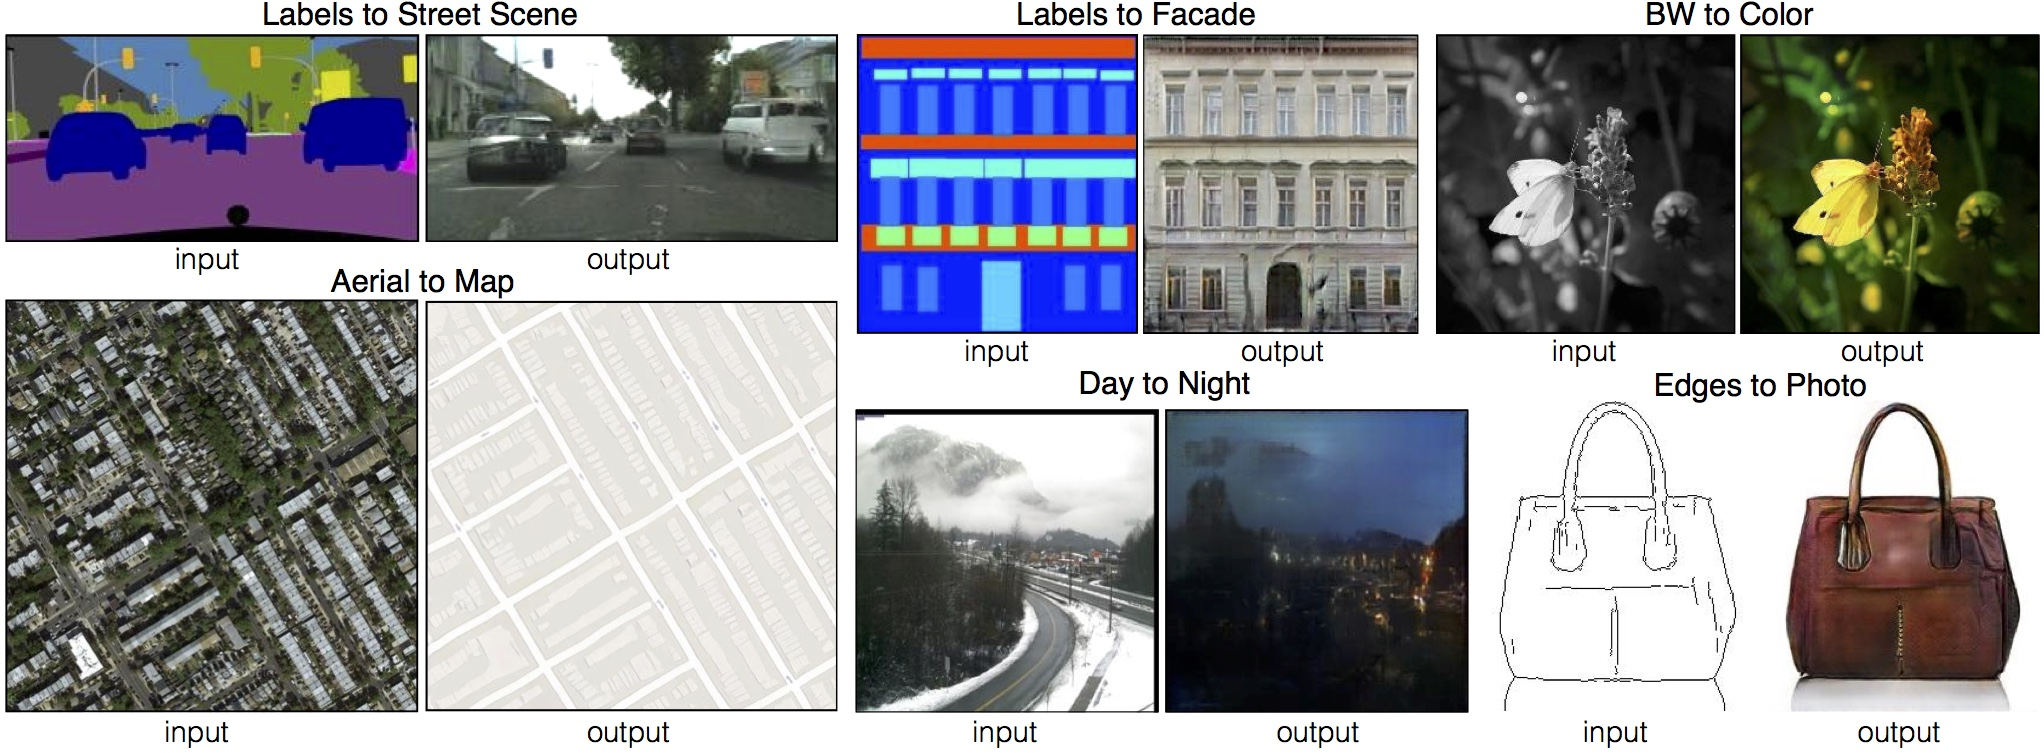
\includegraphics[width=1\linewidth]{pix2pix}
	\end{center}
	
	\captionsetup{width=1\linewidth}
	\caption[Pix2Pix example from \citeauthor{image-to-image}]{Examples from the work of \citeauthor{image-to-image} on image-to-image translation problem \cite{image-to-image}.}
	\label{fig:img-to-img}
	\medskip
	
\end{figure}



\section{Thesis Structure}
%TODO: Finish this

\section{Summary}
In this chapter we introduced the problem of Level Design in video-game industry and the solutions that have been historically applied for approaching the problem. Then we referenced a new area of research in which this work take place and defined its scope.
We also described the main differences between our research domain and the domains of the main contributions in each research area we considered, highlighting the differences between our work and other contributions. In the next chapter we give a more in-depth description of the Generative Adversarial Network models and considerations about the choice of the game. 
